% !TEX root = ../Vorlage_DA.tex
%	########################################################
% 					Bedienungsanleitung
%	########################################################


%	--------------------------------------------------------
% 	Überschrift, Inhaltsverzeichnis
%	--------------------------------------------------------
\chapter{Bedienungsanleitung}


%	--------------------------------------------------------
% 	Suche eines geeigneten Standortes
%	--------------------------------------------------------
\section{Suche eines geeigneten Standortes}
    
    \begin{figure}[H]
            \centering
            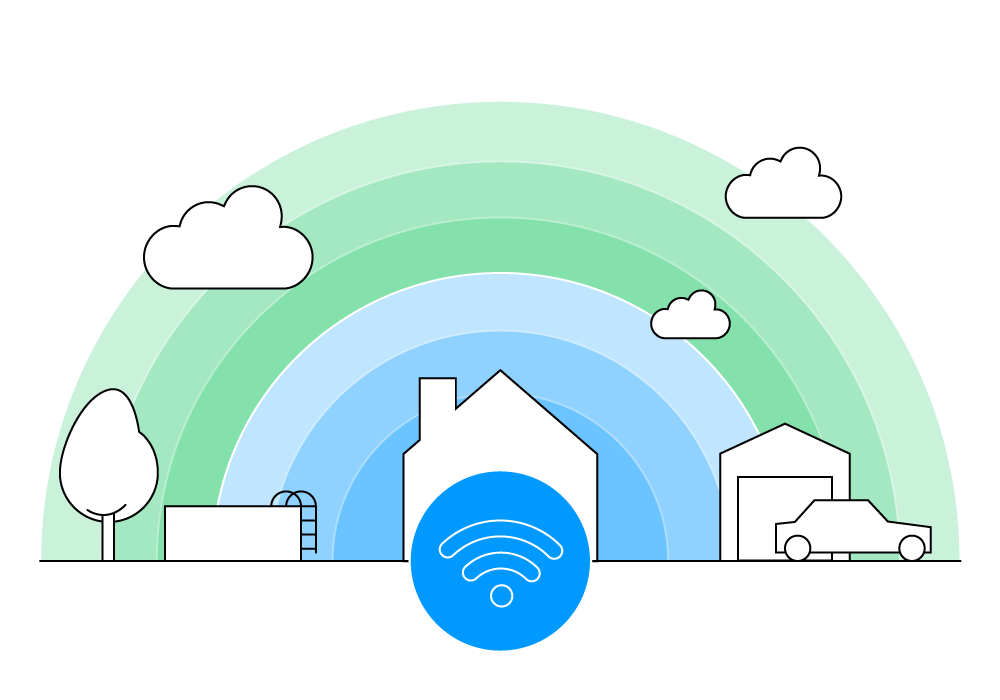
\includegraphics[width=0.8\textwidth]{./media/images/wifirange.png}
            \caption{Atom Screenshot\cite{bib:WiFiBooster}}
            \label{fig:WiFiRange}
    \end{figure}
    
    Damit sunnyHOME überhaupt Daten publizieren kann, braucht die Wetterstation einen Ort mit Verbindung zu einem WLAN-Netz. Handelsübliche WLAN-Netze geben eine mögliche Reichweite von 46 Metern in Gebäuden und 92m im Freien an \cite{bib:WiFiRange}. Diese Werte sind meist jedoch sehr optimistisch. Hat man sunnyHOME im Garten stehen, sollte man mit einer Reichweite von 35-45 Metern rechnen.
    
    Ein Ort mit guter Sonneneinstrahlung ist vorteilhaft.
    
\pagebreak
    
%	--------------------------------------------------------
% 	Einstellen von Ubidots
%	--------------------------------------------------------
\section{Einstellen von Ubidots}
 
    Für das Publizieren der gesammelten Daten wird ein Ubidots-Konto benötigt (siehe: \ref{ref:Ubidots}). Das lässt sich auf ihrer Website \url{www.ubidots.com} machen. Ist man noch Student, kann man sich über \url{www.ubidots.com/education/} ein kostenloses „Education-Konto“ erstellen. 
    
    Ist das Konto erstellt worden, muss ein „Device\footnote{Anleitung „Devices“: https://help.ubidots.com/user-guides/creating-devices-in-ubidots, 07.04.2019}“ erstellt werden. Dann braucht es noch „Variables\footnote{Was sind „Variables“: https://help.ubidots.com/faqs-and-troubleshooting/what-are-variables, 07.04.2019}“ und eine „Dashboard\footnote{Anleitung zu „Dashboards“: https://help.ubidots.com/user-guides/create-dashboards-and-widgets, 07.04.19}“. Sind diese Schritte gemacht, kann das Device wie in Screenshot \ref{fig:ubiDev} aussehen. 
    
    \begin{figure}[H]
            \centering
            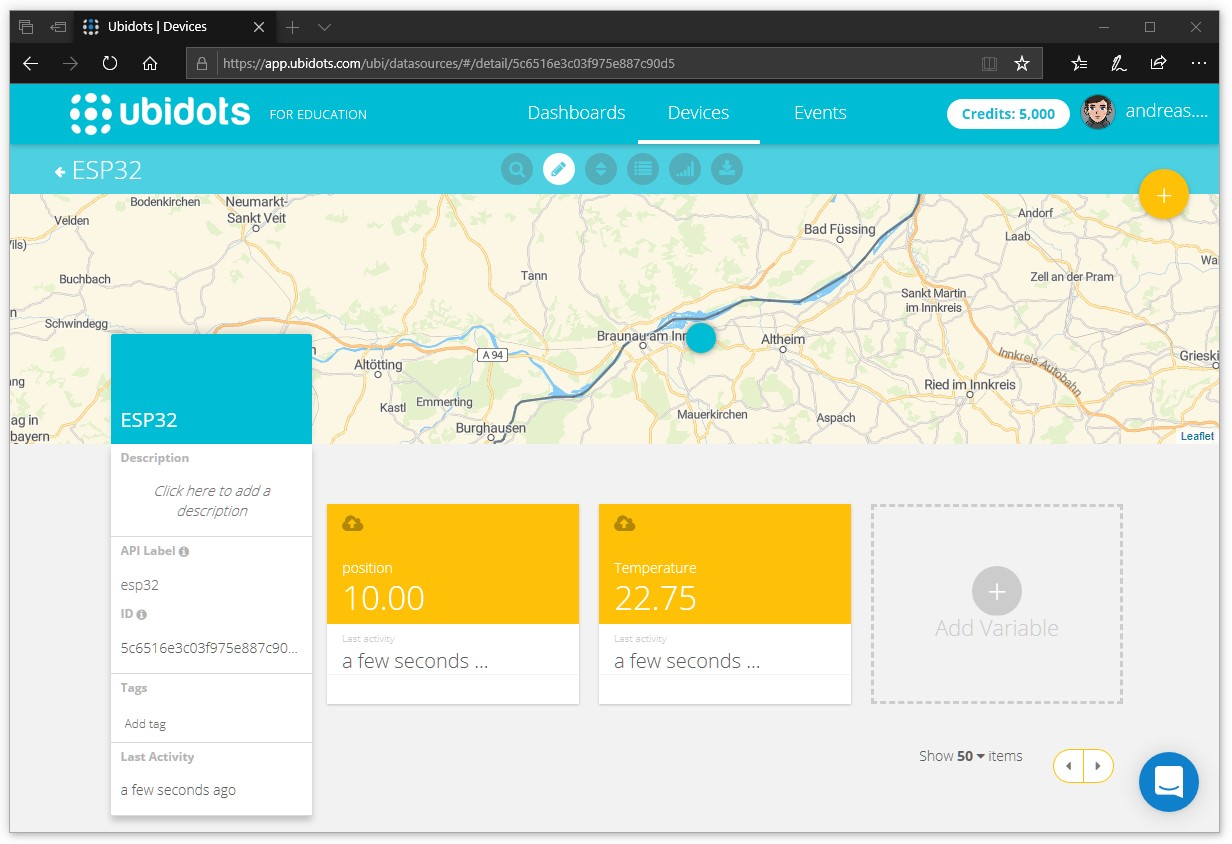
\includegraphics[width=0.8\textwidth]{./media/images/ubidotsDev.jpg}
            \caption{ubidots-Device Screenshot\cite{bib:ubidots}}
            \label{fig:ubiDev}
    \end{figure}
    
\pagebreak
    
%	--------------------------------------------------------
% 	Modifizierung des Codes
%	--------------------------------------------------------
\section{Modifizierung des Codes}
 
    Der letzte Schritt bei der Einrichtung von sunnyHOME, ist das modifizieren des Codes.
    
    Sobald man das Programm in einem passenden Editor (siehe: \ref{ref:Atom}) bzw. in einer passende IDE (siehe: \ref{ref:PlatformIO}) geöffnet hat, sollte die Verbindung zu einem WLAN-Netzwerk hergestellt werden. Im Quellcode befinden sich zwei globale Konstanten, in welche man den Namen seines Netzwerkes und den Schlüssel des Netzwerkes einfügt. In Listing \ref{code:LOGIN} sind diese Konstanten zu sehen. 
    
    \begin{lstlisting}[
            language=c,
            caption={Verbindung mit WLAN-Netzwerk und Ubidots},
            label=code:LOGIN
        ]
///     WLAN Konstanten
#define WIFISSID "meinInternet"         // hier WLAN-SSID eintragen
#define PASSWORD "meinGeheimesPasswort" // hier WLAN-Passworrt eintragen
///     Ubidots Konstanten
#define TOKEN "meinUbidotsToken"        // hier Ubidots-Token eintragen
    \end{lstlisting}
    
    Im nächsten Schritt gilt es die Verbindung zum Ubidots-Broker herzustellen. Wenn man sich ubidots öffnet, findet sich ein Menü-Punkt namens „API Credentials“ (siehe: \ref{fig:ubitoken}). Von dort kopiert man sich den „Default token“, welcher ebenfalls ins Programm eingefügt wird (siehe: \ref{code:LOGIN}).
      
    \begin{figure}[H]
            \centering
            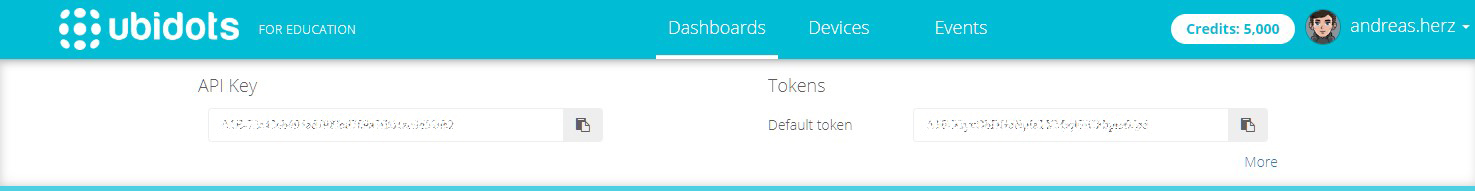
\includegraphics[width=1\textwidth]{./media/images/ubitoken.jpg}
            \caption{Ubidots-token Screenshot\cite{bib:ubidots}}
            \label{fig:ubitoken}
    \end{figure}  
    
    Jetzt fehlen nur noch die Labels. Diese sind Etiketten, welche es für jede Messung, welche über MQTT übertragen werden soll gibt. Für die Labels gibt es ebenfalls globale Konstanten (siehe: \ref{code:label}). 
    
\begin{lstlisting}[
            language=c,
            caption={MQTT-Labels},
            label=code:label
        ]
///   Labels für MQTT
#define VARIABLE_LABEL_TEMP "temperature"   // Hier Temperatur-Label eintragen
#define VARIABLE_LABEL_GPS "gps"            // Hier GPS-Label eintragen
#define DEVICE_LABEL "esp32"                // Hier Device-Label eintragen
    \end{lstlisting}
    
    Wenn die eingetragenen Labels mit den in Ubidots eingetragenen API-Labels identisch sind, sollte die Übertragung der Daten per MQTT nun funktionieren. 

    
    
    
\pagebreak

